\documentclass[conference]{IEEEtran}

\usepackage{amsmath,amssymb,amsfonts}
\usepackage{array}
\usepackage{booktabs}
\usepackage{cite}
\usepackage{graphicx}
\usepackage{hyperref}
\usepackage{xcolor}

\graphicspath{{../../figures/}}

\newcolumntype{P}[1]{>{\raggedright\arraybackslash}p{#1}}

\begin{document}

\title{Maritime Claims Boundary: What Synthetic Low-SNR Evidence Can and Cannot Support in WVF/LF}

\author{\IEEEauthorblockN{J.C.\ Vaught}
\IEEEauthorblockA{Department of Computer Science and Engineering\\
University of South Carolina\\
Columbia, SC, USA}}

\maketitle

\begin{abstract}
The WVF/LF papers motivate their methods with maritime and low-SNR imagery, where horizon lines, small floating objects, and water texture make edge detection genuinely difficult. This paper asks a narrower question: what does the current repository actually support about that maritime motivation, and what does it still not support? Using the source papers, the local synthetic maritime figures, a repeated-trial maritime benchmark, and a source-gap review, we find that the maritime problem framing is credible but bounded. The synthetic evidence shows that large-support classical filters often dominate the repeated-trial summary, while the hard scenes remain hard for all reproduced methods. That result supports the need for careful low-SNR study, but it does not independently validate the source papers' strongest claims about superiority on real aquatic images. The local repository still lacks the four-image aquatic set used in the papers, and the maritime image folder currently contains zero-byte placeholders, so the real-image claim boundary is not merely theoretical. We conclude with more careful wording for the aquatic-domain motivation: the evidence supports maritime scenes as a useful stress test, not as proof of broad method dominance.
\end{abstract}

\begin{IEEEkeywords}
edge detection, maritime imagery, low-SNR, underwater images, reproducibility, claims boundary
\end{IEEEkeywords}

\section{Introduction}
Maritime and underwater scenes are a legitimate edge-detection stress test. Low illumination, nonuniform lighting, absorption, scattering, and water texture can all suppress faint boundaries or fragment meaningful contours~\cite{marques2019,ji2023}. The source WVF/LF papers use exactly that setting to motivate orientation-aware gradient estimation: the thesis and the two IEEE OCEANS papers repeatedly highlight buoy silhouettes, horizons, cables, wave fields, and low-SNR aquatic imagery as examples where conventional derivative filters appear weak~\cite{bagan2023thesis,bagan2024oceans,bagan2025oceans}.

That motivation is plausible. The problem is stronger than the evidence currently available in this repository.
The repository now contains synthetic maritime scenes, repeated seeded trials, and a claims-gap review, but it does \emph{not} contain the real-image benchmark the papers rely on. In particular, the local `datasets/maritime/images` directory consists of zero-byte placeholder files, and the four-image aquatic set described in the papers is not locally available. This paper therefore does not claim to reproduce the source papers' maritime tables. It instead asks a narrower question: what can the synthetic maritime evidence legitimately support, and how should the aquatic-domain claim be written so that it stays inside that boundary?

\section{Evidence Base}
The current repository provides three kinds of evidence relevant to the maritime claim boundary.

First, the source papers themselves supply the conceptual motivation and qualitative examples. The thesis and 2024 paper emphasize horizon lines, buoys, boats, and textured water. The 2025 paper adds the stronger claims: spline-based angle computation, multi-scale and multi-domain fusion, and quantitative superiority on aquatic benchmarks.

Second, the repository contains synthetic maritime scenes that are intentionally hard but controlled. The repeated-trial benchmark generates six scene families: horizon with boat and buoys, cable in water, wave field, underexposed marine scene, dark horizon, and very low SNR waves. Each family is run for ten seeded trials, which gives 60 samples per method overall. That repeated-trial design is important because one-shot synthetic scenes are too noisy to support strong claims.

Third, the repository now contains a source-gap review that makes the missing pieces explicit. The main gaps are unchanged and material: BIPED is absent, the four-image aquatic set is absent, the later multi-scale GMM pipeline is not implemented, and the maritime image folder contains only placeholder files~\cite{sourcegap}. Those absences matter because they determine what can and cannot be claimed about the aquatic domain.

\begin{figure*}[t]
\centering
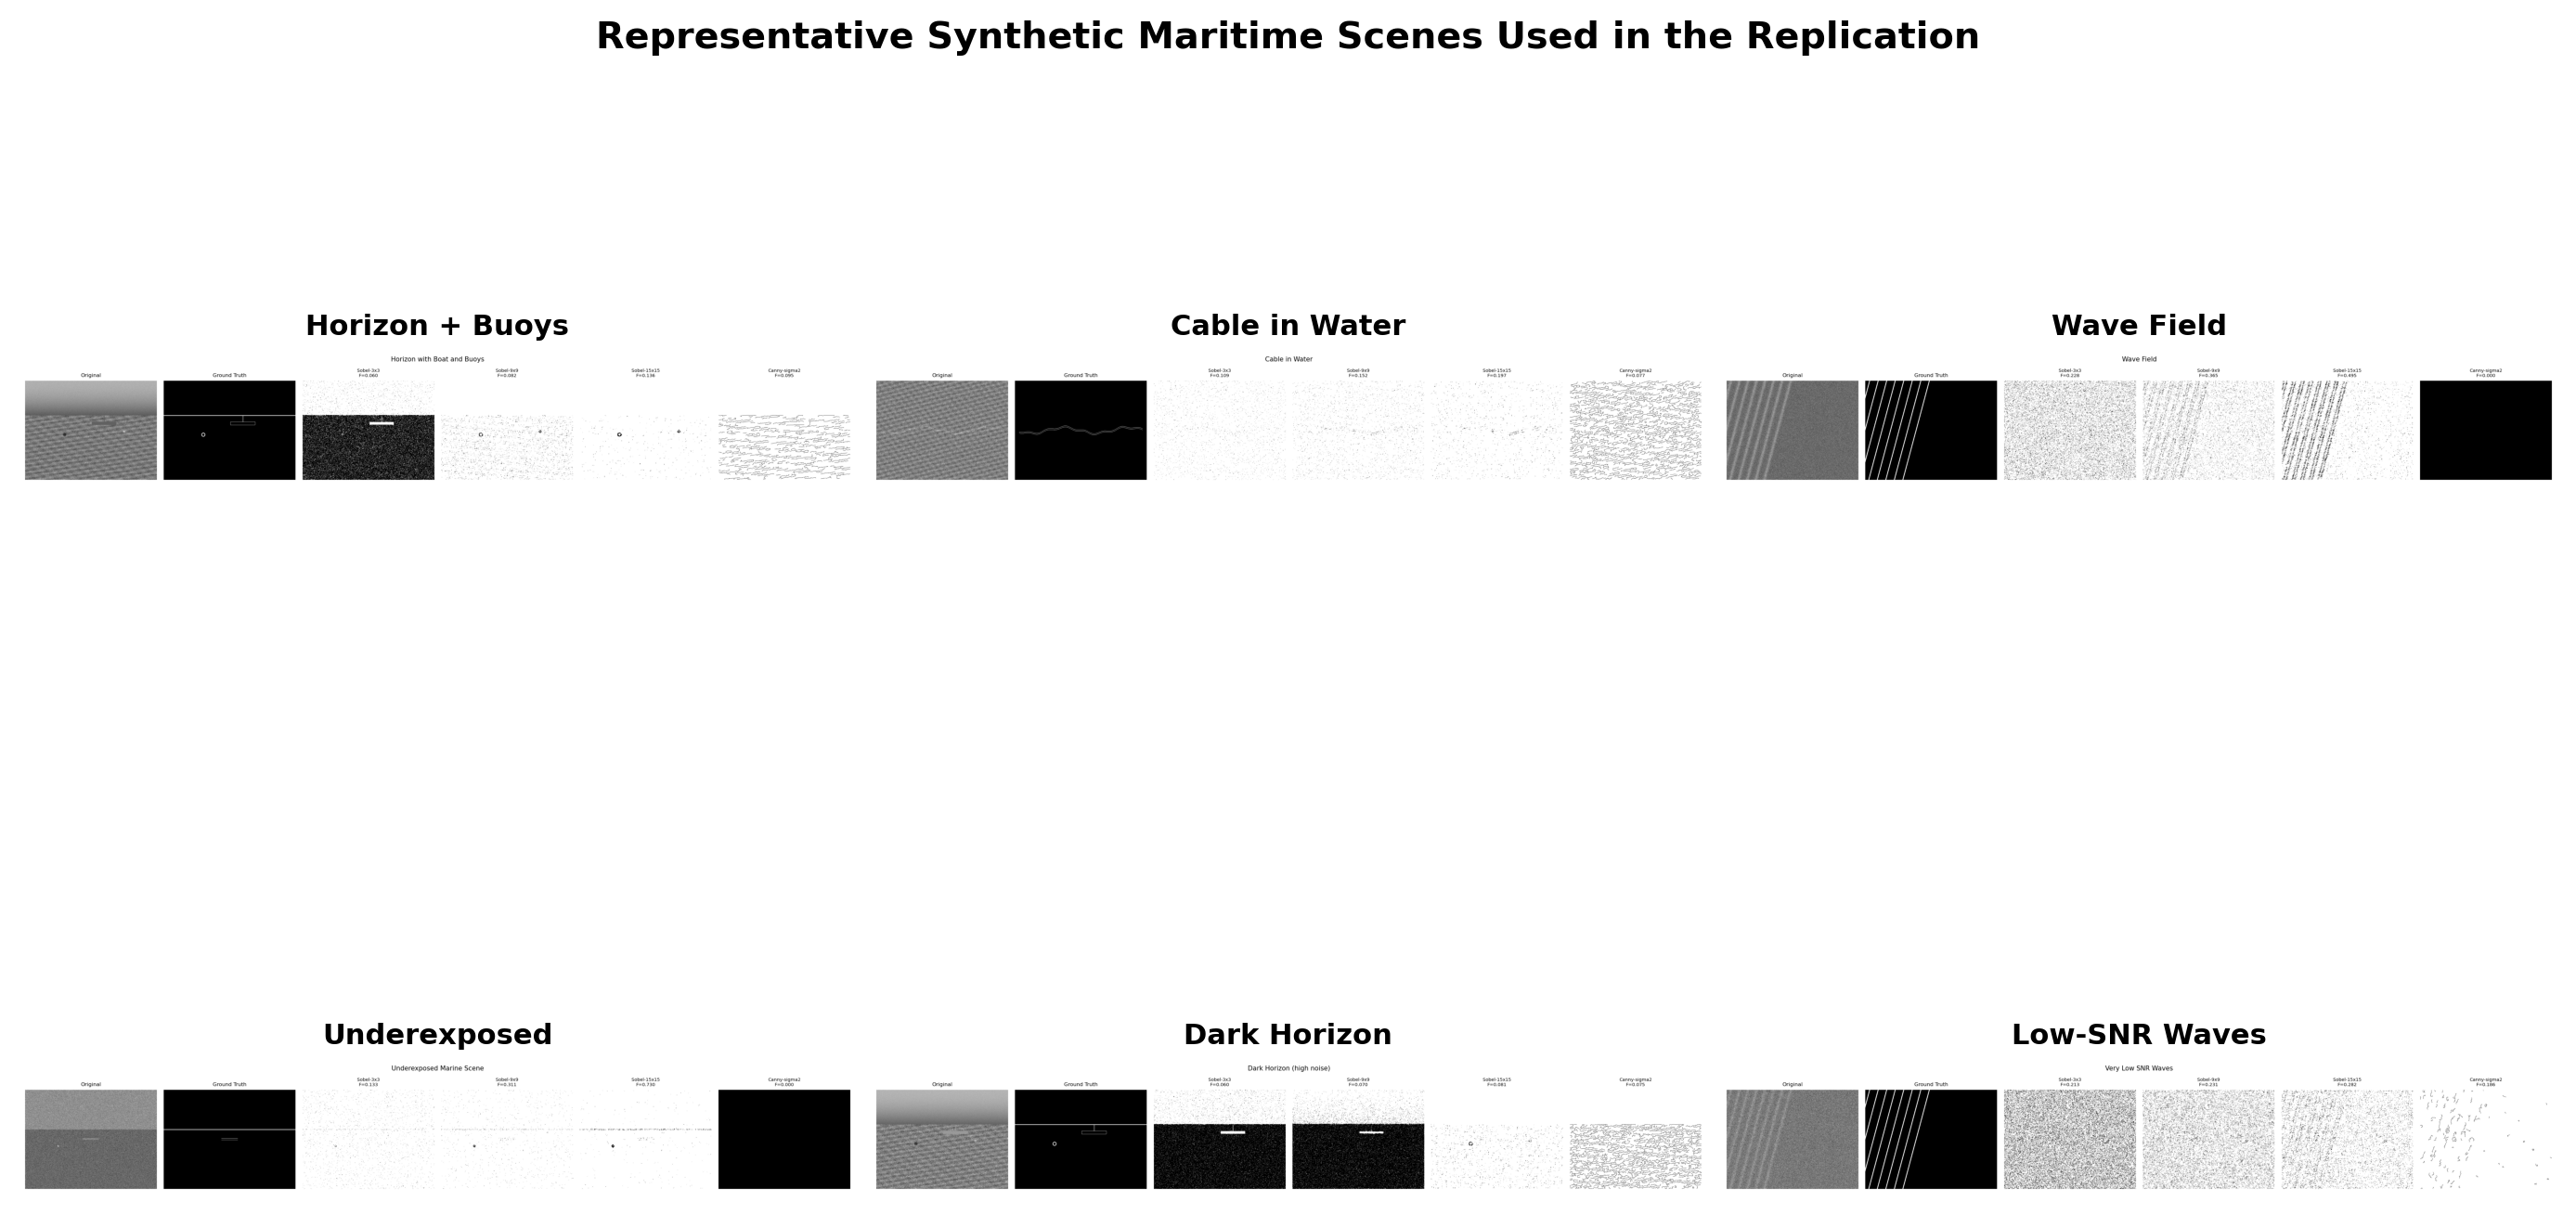
\includegraphics[width=\textwidth]{maritime_scene_montage.png}
\caption{Representative synthetic maritime scenes used in the repeated-trial benchmark. These scenes are useful because they isolate horizon, cable, wave, and underexposure effects, but they are still synthetic stress tests rather than the paper's missing real-image aquatic benchmark.}
\label{fig:montage}
\end{figure*}

\section{Repeated-Trial Maritime Results}
The strongest synthetic evidence is the repeated-trial summary in Fig.~\ref{fig:summary}. The overall ranking is not subtle: large-support Sobel is the best reproduced method by average F-score, followed by Canny with $\sigma=1$, then larger Sobel kernels, with Prewitt and small Sobel variants slightly behind. Table~\ref{tab:overall} lists the aggregate means and 95\% confidence intervals across all 60 samples.

\begin{table}[t]
\centering
\caption{Overall repeated-trial maritime F-scores across 60 samples}
\label{tab:overall}
\scriptsize
\begin{tabular}{P{2.5cm}rr}
\toprule
Method & Mean F-score & 95\% CI \\
\midrule
Sobel 15$\times$15 & 0.3364 & 0.0565 \\
Canny $\sigma=1$ & 0.2540 & 0.0692 \\
Sobel 9$\times$9 & 0.2128 & 0.0285 \\
Sobel 7$\times$7 & 0.1645 & 0.0202 \\
Prewitt 3$\times$3 & 0.1416 & 0.0167 \\
Sobel 3$\times$3 & 0.1363 & 0.0167 \\
Sobel 5$\times$5 & 0.1318 & 0.0177 \\
Canny $\sigma=2$ & 0.0702 & 0.0154 \\
\bottomrule
\end{tabular}
\end{table}

\begin{figure*}[t]
\centering
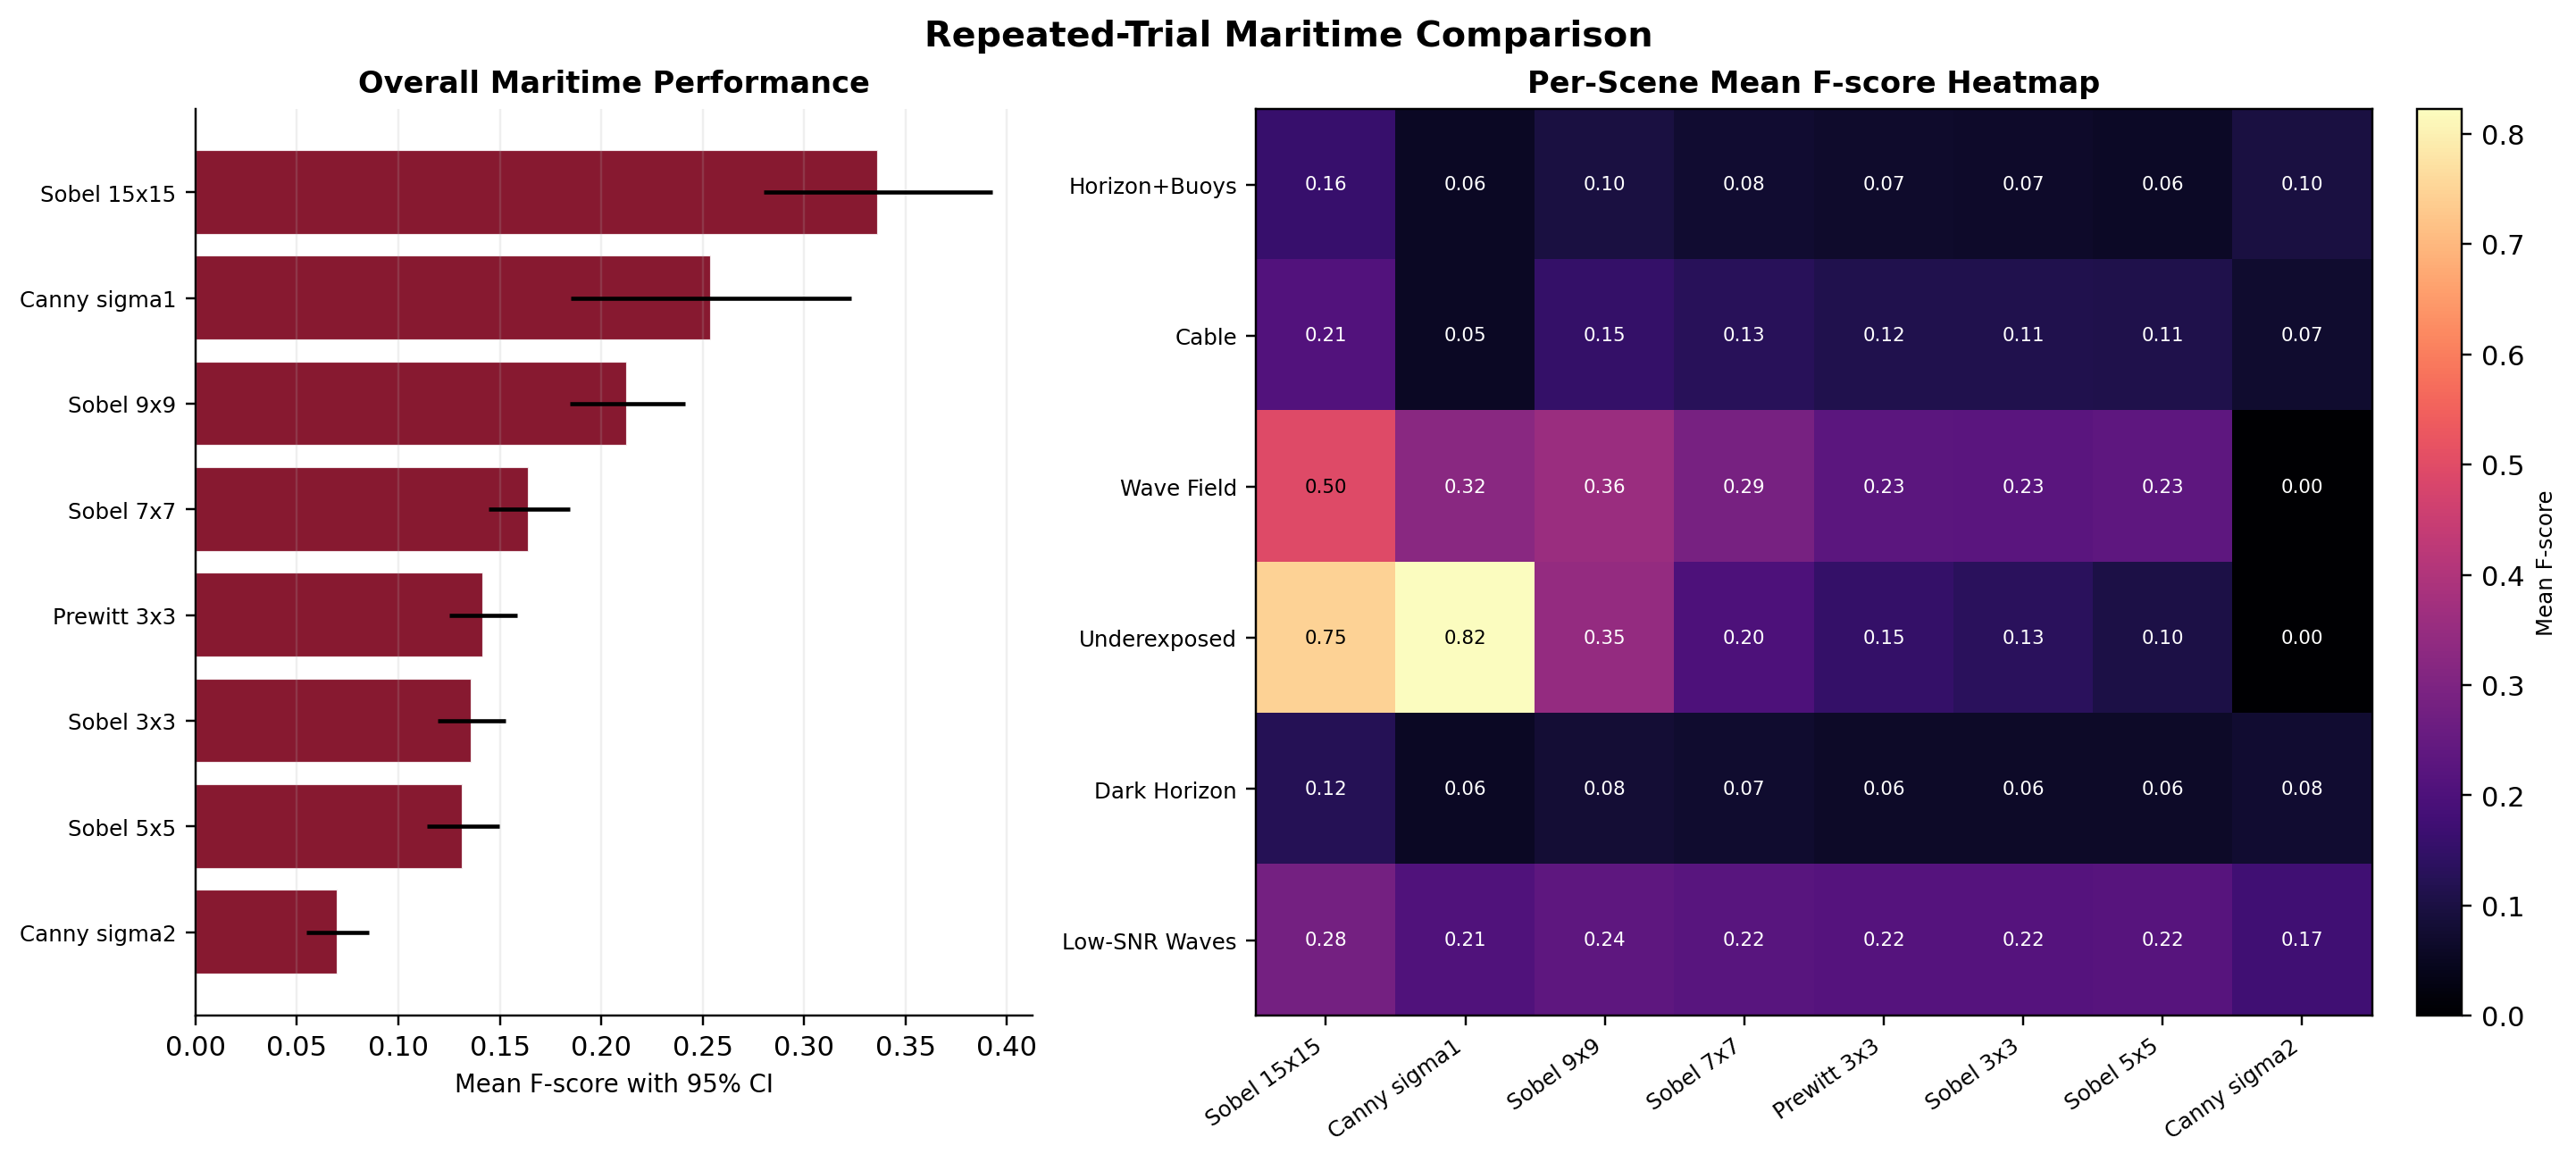
\includegraphics[width=\textwidth]{maritime_summary.png}
\caption{Repeated-trial maritime comparison. The left panel shows the overall mean F-score with 95\% confidence intervals; the right panel is a per-scene heatmap. The figure supports the need for maritime stress testing, but it does not support a blanket claim that the WVF/LF family dominates conventional filters on the reproduced benchmark.}
\label{fig:summary}
\end{figure*}

The scene-level structure is more important than the aggregate ranking. The underexposed marine scene is the strongest case for a sparse, low-threshold detector such as Canny $\sigma=1$, which reaches 0.8225 mean F-score there. But that same method is unstable overall, and the other scenes tell a different story. Wave fields strongly favor the large-support Sobel family, with Sobel 15$\times$15 at 0.4980 mean F-score. The cable-in-water scene also favors Sobel 15$\times$15 at 0.2112. The dark-horizon scene is weak for every method, with all methods clustered below 0.13. That pattern is exactly what a bounded maritime stress test should show: the domain is hard, but the winner changes by scene family, and no single conventional detector is universally dominant.

This matters for the source papers because their maritime examples are often discussed as if the low-SNR setting itself justifies broad superiority claims. The repeated-trial summary does not support that move. It supports a more careful statement: maritime scenes are a meaningful adversarial setting, and different edge operators react differently to scene structure, but the synthetic benchmark here does not certify a general WVF/LF win.

\section{What The Evidence Supports}
The local evidence supports three restrained claims.

First, the maritime setting is real. The synthetic scenes are not trivial, and they capture the same qualitative problems the source papers emphasize: horizon ambiguity, small objects, cable-like curves, wave texture, and underexposure. That makes the research motivation credible.

Second, support size matters. Across the repeated-trial benchmark, larger-support classical filters often improve over small $3\times3$ baselines. This is consistent with the intuition behind WVF/LF: larger local support can recover structure that tiny kernels miss. The synthetic data therefore supports the \emph{problem framing} even when it does not support the \emph{method superiority} claim.

Third, the evidence is bounded by the data that are actually available. The repository does not have the paper's four-image aquatic set, does not have BIPED, and does not have the later multi-scale GMM pipeline. Those are not minor omissions. They prevent a direct validation of the strongest aquatic-domain claims, including the real-image edge maps and the later spline-angle demonstrations.

\section{What The Evidence Does Not Support}
The current repository does \emph{not} support the strongest form of the aquatic-domain claim.

It does not show that WVF/LF is superior on real maritime imagery, because the real maritime image folder is empty of usable image data. It does not show that the four-image aquatic benchmark from the papers can be reproduced locally, because that dataset is unavailable here. It does not show that the later multi-scale, multi-domain, GMM-based pipeline has been independently verified, because that pipeline is not implemented.

Just as important, the synthetic maritime benchmark does not justify collapsing all maritime scenes into one conclusion. The same method can look strong on an underexposed scene and weak on a dark horizon or wave field. A careful paper must preserve that variation instead of smoothing it away.

\section{How The Claim Should Be Written}
The aquatic-domain motivation should be rewritten as a bounded claim, not a universal one.

A defensible formulation is: maritime and low-SNR scenes are a plausible and practically relevant stress test for edge detection; controlled synthetic scenes show that scene structure can strongly affect detector behavior; and larger-support orientation-aware operators can help in some such conditions, but the repository does not yet contain enough real-image evidence to claim broad superiority or deployment readiness.

That wording is less dramatic than the source papers, but it is more accurate.
It leaves room for the idea that WVF/LF may still be useful in the maritime domain, while refusing to overstate what the current evidence proves. It also makes the missing data an explicit part of the scientific statement rather than an implicit footnote.

\section{Conclusion}
The synthetic maritime evidence is useful, but it is bounded evidence. It demonstrates that maritime edge detection is hard, that scene family matters, and that larger-support classical filters can be strong in this domain. It does \emph{not} independently validate the source papers' broad aquatic superiority claims, because the repository lacks the real-image aquatic benchmark, lacks BIPED, and lacks the later multi-scale GMM pipeline. Until those gaps are closed, the most honest maritime claim is a stress-test claim: the aquatic domain is a meaningful adversarial setting for edge detection, but the current repository only supports a cautious, not a triumphant, interpretation.

\begin{thebibliography}{99}

\bibitem{bagan2023thesis}
L.~Bagan, ``Wide view and line filter for enhanced image gradient computation and edge determination,'' M.S.\ thesis, Univ.\ South Carolina, 2023.

\bibitem{bagan2024oceans}
L.~Bagan and Y.~Wang, ``Wide view and line filter for enhanced gradient computation in aquatic environment,'' in \textit{Proc.\ IEEE OCEANS}, 2024.

\bibitem{bagan2025oceans}
L.~Bagan and Y.~Wang, ``Multi-scale and multi-domain edge determination with accurate gradient orientation computation in aquatic environment,'' in \textit{Proc.\ IEEE OCEANS}, 2025.

\bibitem{marques2019}
T.~P.~Marques, A.~B.~Albu, and M.~Hoeberechts, ``A contrast-guided approach for the enhancement of low-lighting underwater images,'' \textit{Journal of Imaging}, vol.~5, no.~10, p.~79, 2019.

\bibitem{ji2023}
K.~Ji, W.~Lei, and W.~Zhang, ``A deep Retinex network for underwater low-light image enhancement,'' \textit{Machine Vision and Applications}, vol.~34, art.\ no.~122, 2023.

\bibitem{sourcegap}
J.~C.~Vaught, ``Source paper gap review,'' \texttt{results/source\_paper\_gap\_review.md}, 2026.

\bibitem{canny1986}
J.~Canny, ``A computational approach to edge detection,'' \textit{IEEE Trans.\ Pattern Anal.\ Mach.\ Intell.}, vol.~8, no.~6, pp.~679--698, 1986.

\bibitem{dexined2023}
X.~Soria, E.~Riba, and A.~D.~Sappa, ``Dense extreme inception network for edge detection,'' \textit{Pattern Recognition}, vol.~139, 2023.

\bibitem{teed2023}
X.~Soria, Y.~Li, M.~Rouhani, and A.~D.~Sappa, ``Tiny and efficient model for the edge detection generalization,'' in \textit{Proc.\ IEEE ICCVW}, 2023.

\end{thebibliography}

\end{document}
